\subsection{HotpotQA 环境}
\label{subsec:hotpotqa}
我们还在 HotpotQA 上进一步评估了该框架。在这一任务中，主要性能瓶颈来自信息检索延迟。具体来说，智能体需要通过顺序调用 Wikipedia API 来回答多跳问题\cite{yang2018hotpotqadatasetdiverseexplainable}。这种工具调用模式与现实世界中每轮往返都具有较高网络延迟的智能体工作流非常相似。我们采用\cref{framework}中的框架：当真实 API 调用仍在执行时，Speculator 预测可能的 Wikipedia 内容。借助这种并行性，智能体不必阻塞等待 API 返回，而可以基于暂定信息继续推理。

\subsubsection{实验设置}
我们在 ReAct\cite{yao2023reactsynergizingreasoningacting} 的基础上构建框架；ReAct 会交替进行思维链推理与工具使用。

\textbf{推测流水线。} 在这个场景中，状态 $s_t$ 由完整的推理轨迹历史以及已经检索到的信息（即 API 响应）组成。在每个时间步，Actor 接收当前状态 $s_t$，选择一个 API 调用 $h_t \in\{\text{Search(), Lookup(), Finish()}\}$ 及其对应参数 $q_t$，例如 \texttt{Search(entity)}。调用 $h_t(q_t)$ 会返回一个响应 $a_t$，通常提供与查询实体相关的信息。我们的推测框架按如下方式工作：
\begin{enumerate}[leftmargin=*]
    \item Speculator 预测 API 调用响应 $\hat{a}_t^{(i)}$，从而得到预测的下一状态 $\hat{s}_{t+1}^{(i)} = f(s_t,\hat{a}_t^{(i)})$，其中 $i\in\{1,\dots,k\}$。
    \item 基于这些状态，Actor 会生成推理轨迹，并进一步决定下一次 API 动作 $(\hat{h}_{t+1}^{(i)}, \hat{q}_{t+1}^{(i)})$，其中 $i\in\{1,\dots,k\}$。
\end{enumerate}

\textbf{评估。}
我们通过预测得到的 API 决策 $(\hat{h}_{t+1}, \hat{q}_{t+1})$ 的准确率来评估推测流水线的有效性。具体而言，我们将预测调用与在真实响应 $a_t$ 下得到的真实调用 $(h_{t+1}, q_{t+1})$ 进行比较。我们采用严格匹配标准：只有当 $\hat{h}_{t+1} = h_{t+1}$ 且 $\hat{q}_{t+1} = q_{t+1}$ 时，才计为正确。这个严格标准能够准确反映推测是否真的带来了有效推进；即便只是参数表达上的细微差别（如同义词或词序不同），也会被判定为不匹配。

\textbf{智能体配置。}
我们在三种 Speculator 模型上评估推测准确率：GPT-5-nano、GPT-4.1-nano 和 Gemini-2.5-flash。对每种模型，我们都测量 top-$k$ 预测准确率，其中 $k \in \{1,3\}$。

\subsubsection{结果}

\begin{wrapfigure}{r}{0.45\columnwidth}
\vspace{10pt}
    \centering
    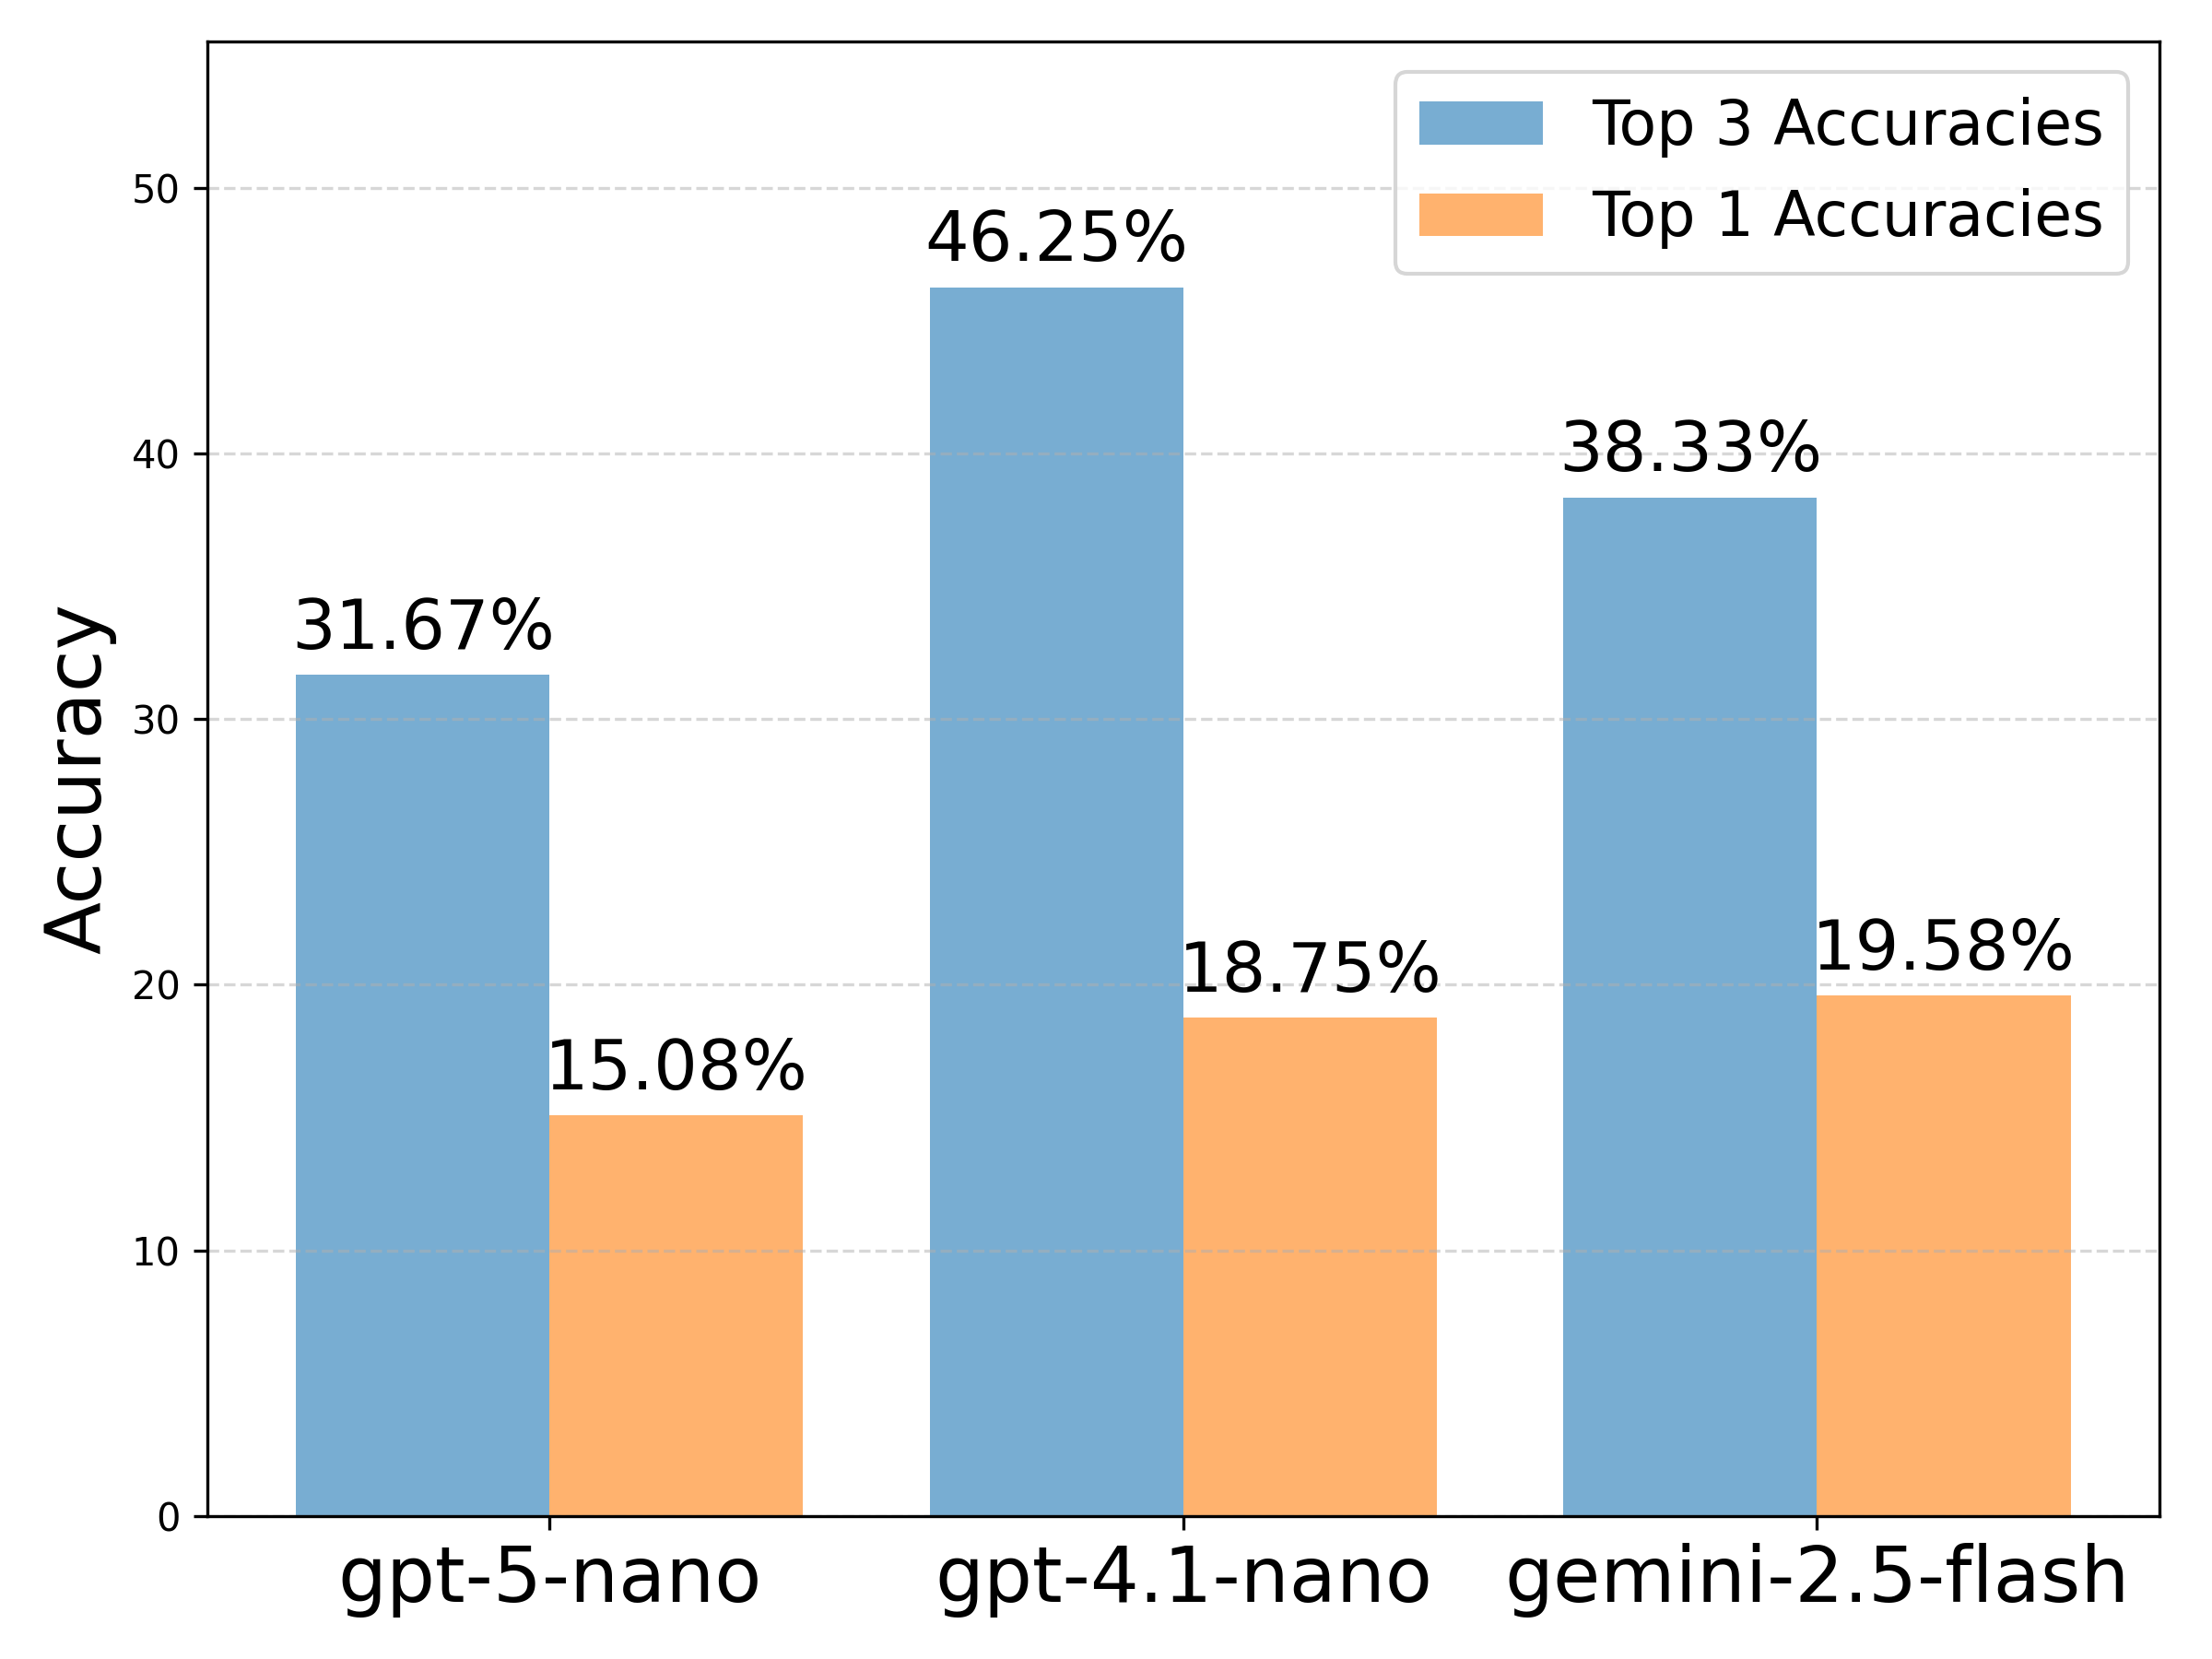
\includegraphics[width=\linewidth]{figures/hotpotqa/accs_gemini-2.5-flash.png}
    \caption{以 gemini-2.5-flash 作为 Actor 时的准确率。与只预测单个动作相比，推测多个动作（$k=3$）会得到更高准确率。}
    \label{fig:hotpotqa_accs}
\end{wrapfigure}

\cref{fig:hotpotqa_accs} 表明，尽管我们采用了严格匹配标准，Speculator 在 top-3 预测下仍能以最高 $46\%$ 的概率预测中真实 API 调用。与 top-1 相比，top-3 的准确率有明显提升，这说明只要适度增加推测宽度，就能带来显著的准确率收益。我们的推测机制之所以有效，是因为它可以在原本等待 API 返回的空闲时间里，预先计算后续推理路径。

\textbf{模型模式。}
我们观察到，不同 Speculator 在 API 决策上存在较大差异，这主要来自措辞层面的不同——有些模型的调用表述更简洁，有些则更倾向于过度具体化。有趣的是，更强的模型有时反而准确率更低，因为它们更容易给出多样化且强上下文依赖的查询（例如 “List of Nobel laureates in physics 1970s” 与 “1970s Nobel Prize Physics winners list”），而在严格匹配标准下，这些差异都会受到惩罚。相比之下，较弱的模型往往输出更简单、也更可预测。
